\documentclass[border=10pt]{standalone}
\usepackage{pgfplots, tikz}
\usetikzlibrary{fadings}
\pgfplotsset{width=20cm,compat=1.9}

\begin{document}
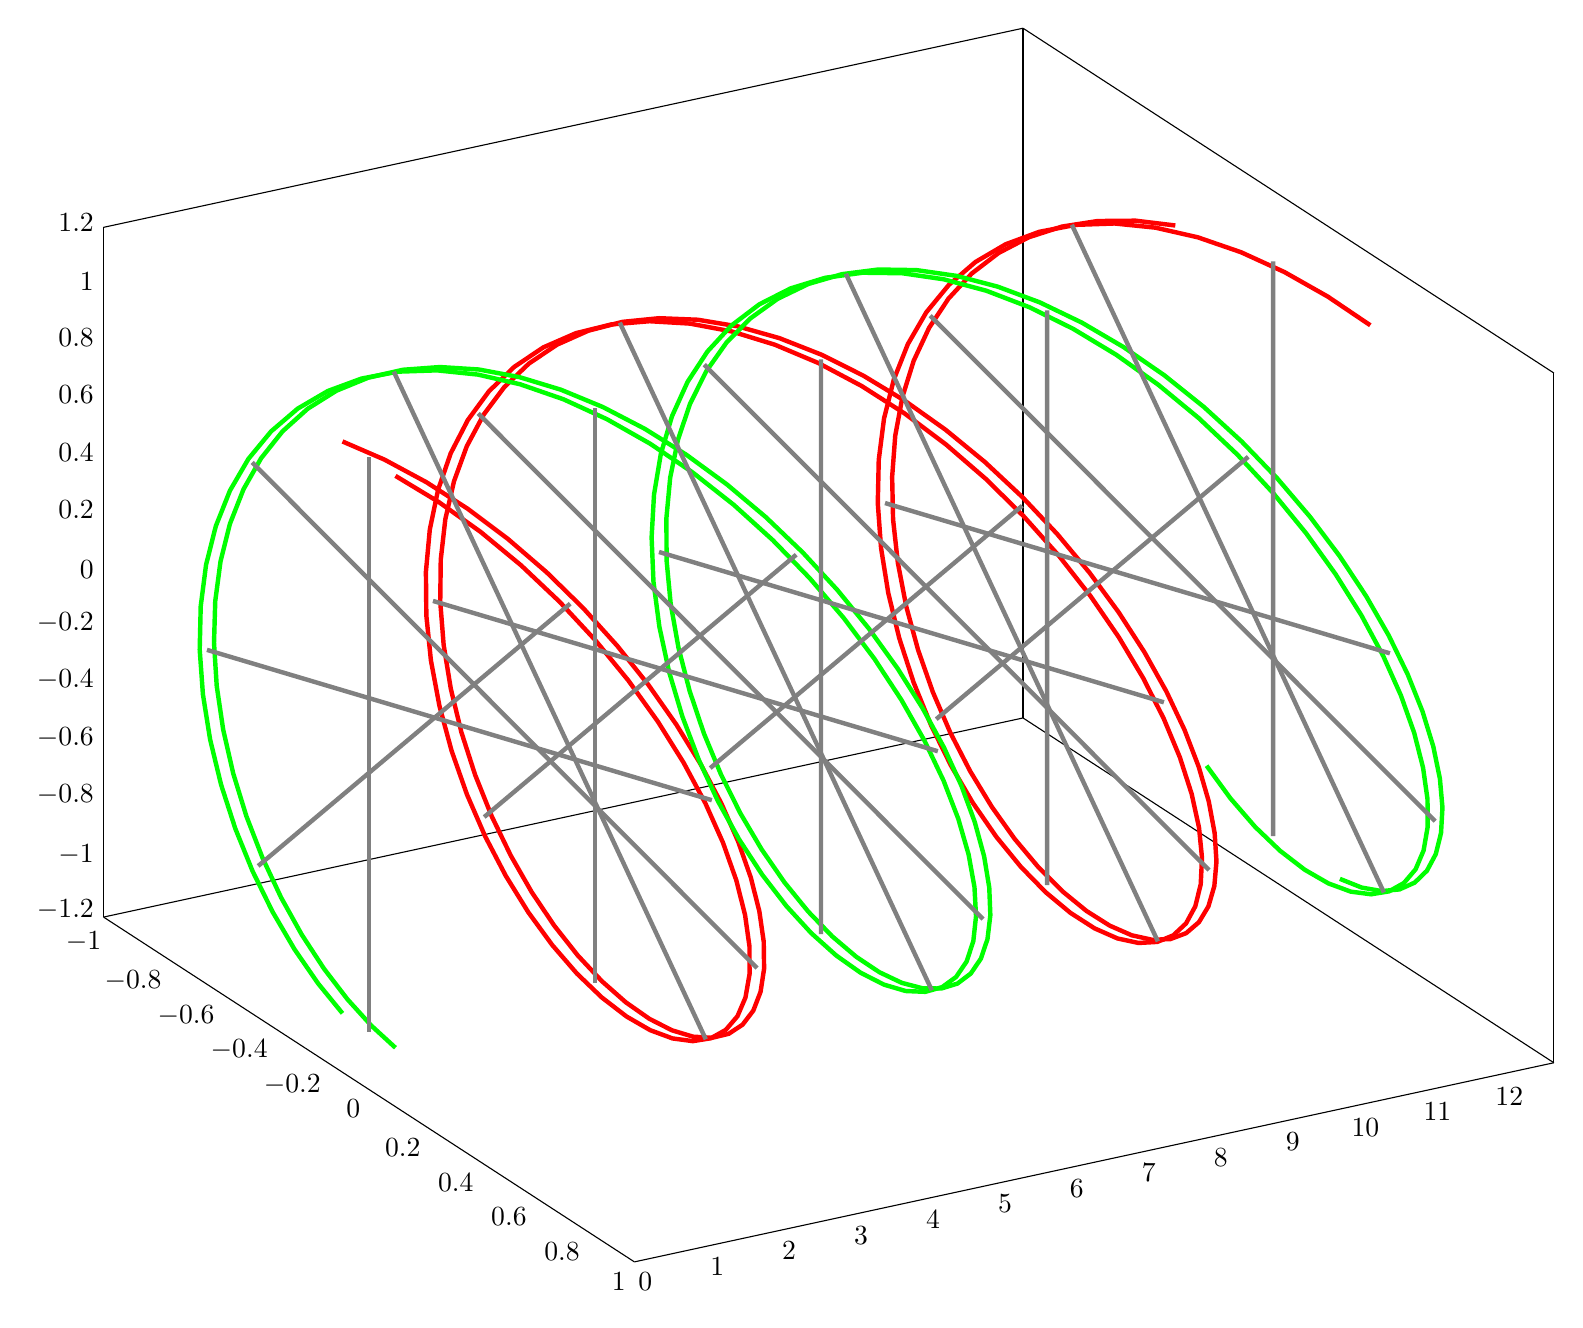
\begin{tikzpicture}
  \tikzfading[name=fade down,top color=blue!0, bottom color=red!100]
  \tikzfading[name=fade up,top color=red!100, bottom color=blue!0]
  \begin{axis}
    [
    % x=1cm,
    % y=1cm,
    % axis line style={draw=none},
    % axis line style={draw opacity=0},
    tick style={draw opacity=0},
    view={60}{30},
    ]
\addplot3[
    domain=0.1:4.1*pi,
    samples = 100,
    samples y=0,
    color=red,
    style=ultra thick
]
({sin(deg(x))},
{x-0.1},
{cos(deg(x))}
);
\addplot3[
    domain=-0.1:3.9*pi,
    samples = 100,
    samples y=0,
    color=red,
    style=ultra thick
]
({sin(deg(x))},
{x+0.1},
{cos(deg(x))}
);
\addplot3[
    domain=pi-0.1:4.9*pi,
    samples = 100,
    samples y=0,
    color=green,
    style=ultra thick,
]
({sin(deg(x))},
{x-pi+0.1},
{cos(deg(x))}
);
\addplot3[
    domain=pi+0.1:5.1*pi,
    samples = 100,
    samples y=0,
    color=green,
    style=ultra thick,
]
({sin(deg(x))},
{x-pi-0.1},
{cos(deg(x))}
);
\pgfplotsinvokeforeach{0,1,...,20} {
\addplot3[color=gray, style=ultra thick] coordinates {({sin(deg(2*pi/10*#1))}, {2*pi/10*#1}, {cos(deg(2*pi/10*#1))}) ({sin(deg(2*pi/10*#1-pi))}, {2*pi/10*#1}, {cos(deg(2*pi/10*#1-pi))})};
}

%\addplot3 coordinates {({sin(deg(\k))}, {\k}, {cos(deg(\k))}) ({sin(deg(\k-pi))}, {\k}, {cos(deg(\k-pi))})};
% \addplot3 coordinates {(0, pi, -1) (0, pi, 1)};
\end{axis}
\end{tikzpicture}
\end{document}